\chapter{Acesso ao Moodle da UFPB Virtual}
Neste capítulo apresentaremos como professores e tutores poderão acessar o Moodle da UFPB Virtual, e como deverão prosseguir na navegação do mesmo.
\section{Informações importantes}
O acesso ao Ambiente de Educação à Distância pode ser feito de duas formas: ou diretamente no sítio \url{http://www.ead.ufpb.br}, ou 
clicando no botão \textbf{Acesso ao Moodle EAD} na página da UFPB Virtual \url{http://portal.virtual.ufpb.br}, como apresentado na Figura \ref{fig:apresentacao}.

\begin{figure}[htbp]
 \begin{center}
 \fbox{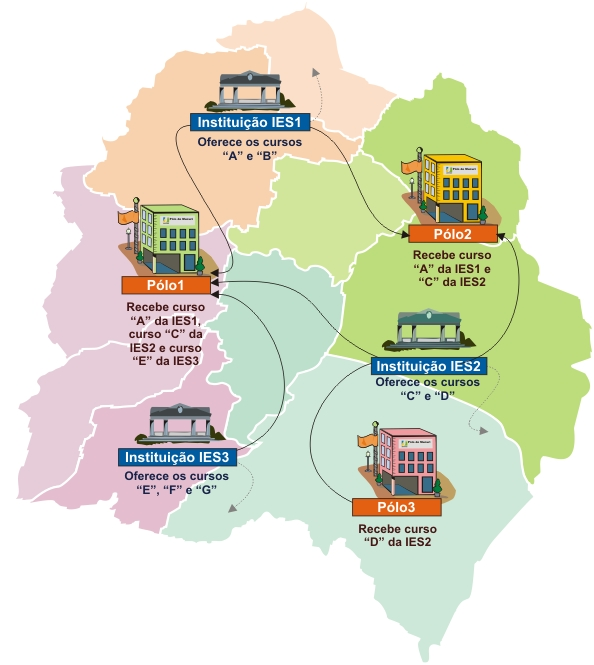
\includegraphics[width=0.5\textwidth]{imagem/cap2/fig1.jpg}}
  \caption{Site da UFPB Virtual}
  \label{fig:apresentacao}
 \end{center}
\end{figure}

Após o acesso pode-se também adicionar o site aos Favoritos do navegador, para que o endereço possa ser revisitado rapidamente. 
Estando na página de acesso do Moodle, basta clicar em  Favoritos, no menu do navegador.

Ao utilizar algum serviço de busca na Internet, como o Google, Yahoo, Ask, Bing, etc, deve-se ter o cuidado de verificar se o endereço acessado é o mesmo mencionado acima, pois os resultados da busca podem trazer também outras plataformas da UFPB Virtual, cujos cadastros não são compartilhados. Por exemplo, os sites do Moodle Presencial e do Moodle Pós-Graduação.
\section{Fazendo login}
\label{chap2:sec:login}
\index{Login}
A página de acesso o conteúdo da plataforma virtual está illustrada na Figura \ref{fig:login}. Em particular, para acessar o  

Para o acesso do conteúdo exposto na plataforma virtual é necessário a realização do login.
Para isso é necessário o preenchimento de dois campos obrigatórios pelo usuário, illustrados 
na Figura~\ref{fig:login}: o Nome de usuário e a Senha.

\begin{figure}[htbp]
 \begin{center}
 \fbox{\includegraphics[width=0.8\textwidth]{imagem/cap2/fig2.jpg}}
  \caption{Página de acesso a Plataforma}
  \label{fig:login}
 \end{center}
\end{figure}

No Ambiente Virtual da UFPB, o cadastro dos usuários é realizado de tal forma que cada usuário tenha somente 
um cadastro. Para isso, os alunos utilizam como nome de usuário o \emph{número de matrícula}, os tutores o \emph{número de CPF} (Cadastro de Pessoa Física), enquanto que os professores e os coordenadores de pólo e curso o seu \emph{número de SIAP} (Sistema Integrado de Administração de Pessoal).

Para os usuários que acessam a plataforma pela primeira vez, o procedimento adotado é o preenchimento do campo Senha com a mesma informação utilizada para o campo Nome de Usuário. Por exemplo, um tutor que acessa a plataforma pela primeira vez deverá 
usar o seu CPF tanto como Login como a sua Senha.
\section{Trocando a senha}
\label{chap2:sec:trocando}
\index{Trocando senha}
Como visto na Seção~\ref{chap2:sec:login}, o usuário em seu primeiro acesso utilizará como senha o seu nome de usuário. Por motivos de segurança estes serão redirecionados para uma nova página, como pode ser visto na Figura \ref{fig:modifica senha}, em que necessitará o preenchimento de três campos. O campo \textbf{Senha atual} que corresponde ao nome de usuário utilizado, o campo \textbf{Nova senha} que deverá ser preenchido com a senha que o usuário adorará para acessar plataforma, não podendo ser igual ao nome de usuário, e o terceiro e último campo que requer a repetição da informação fornecida no campo \textbf{Nova senha}.

\begin{figure}[htbp]
 \begin{center}
 \fbox{\includegraphics[width=0.6\textwidth]{imagem/cap2/fig3.jpg}}
  \caption{Página de modificação de senha}
  \label{fig:modifica senha}
 \end{center}
\end{figure}

Da mesma forma o usuário poderá atualizar sua senha, através do menu \textbf{Configurações} na seção \textbf{Minhas configurações de perfil}, como destacado na Figura \ref{fig:menu senha}.

\begin{figure}[htbp]
 \begin{center}
 \fbox{\includegraphics[width=0.3\textwidth]{imagem/cap2/fig4.jpg}}
  \caption{Menu para modificação de senha pelo usuário}
  \label{fig:menu senha}
 \end{center}
\end{figure}

\section{Recuperando a senha}
\index{Recuperando senha}
Caso o usuário tenha esquecido sua senha ou seu nome de usuário, a recuperação pode ser realizada através do link \textbf{Esqueceu o seu nome de usuário ou a sua senha? }disposto abaixo do campo \textbf{Senha} na página principal da plataforma, como visto na Figura \ref{fig:login}. Ao acessar este link, o usuário será direcionado para a página representada na Figura \ref{fig:recupera senha}.

\begin{figure}[htbp]
 \begin{center}
 \fbox{\includegraphics[width=0.6\textwidth]{imagem/cap2/fig5.jpg}}
  \caption{Página de recuperação de senha}
  \label{fig:recupera senha}
 \end{center}
\end{figure}
Nesta página há dois campos: \textbf{Nome de usuário} e \textbf{Endereço de e-mail}, que não necessita de preenchimento simultâneo, sendo apenas necessário um com a informação cadastrada no sistema Moodle. Caso o usuário informe o nome de usuário ou e-mail, é necessário que em seu cadastro o campo e-mail esteja preenchido corretamente, já que uma senha temporária será enviada a este e-mail. A senha temporária lhe dará acesso à plataforma e pedirá o usuário por uma nova senha da mesma forma descrita na Seção~\ref{chap2:sec:trocando}. 
Caso o usuário encontre dificuldades em realizar essa operação, o mesmo deve entrar em contato com o suporte através do e-mail \url{suporte@virtual.ufpb.br}, informando seus dados e informando o ocorrido.

\section{Guia de navegação no Moodle}
Ao entrar no ambiente o usuário visualizará a página inicial do Moodle, como illustrada na Figura \ref{fig:inicio}.

\begin{figure}[htbp]
 \begin{center}
 \fbox{\includegraphics[width=0.6\textwidth]{imagem/cap2/fig6.jpg}}
  \caption{Página inicial}
  \label{fig:inicio}
 \end{center}
\end{figure}
A página inicial do Moodle possui duas colunas. Do lado esquerdo os blocos geralmente relacionados à configuração do Moodle e os blocos de conteúdo geral. Na coluna da direita, mais ampla, se encontram informações institucionais e acadêmicas e, abaixo dessas, a lista dos cursos aos quais o usuário está vinculado. Essa página varia um pouco conforme a \emph{função} do usuário no ambiente.

\begin{figure}[htbp]
 \begin{center}
 \fbox{\includegraphics[width=0.3\textwidth]{imagem/cap2/fig7.jpg}}
  \caption{Configurações disponíveis}
  \label{fig:conf disp}
 \end{center}
\end{figure}


Como função pode-se entender o nível de permissões que o usuário possui. Um professor verá mais funcionalidades e recursos que um tutor, que por sua vez tem mais privilégios que um estudante. No entanto, o padrão descrito acima vale para qualquer tipo de usuário. As configurações disponíveis para um professor ou tutor são de alteração do perfil e gerenciamento das mensagens. A Figura~\ref{fig:conf disp} apresenta algumas das configurações disponíveis.


O perfil público do usuário também pode ser acessado clicando no seu nome, no alto de qualquer página do lado direito, dessa forma é possível acessar seu perfil o que permite edições do perfil, etc. Do lado esquerdo vê-se o \textbf{Calendário} e, eventualmente, o \textbf{bloco de últimas notícias}, como demonstrado na seguinte Figura.

\begin{center}
 \fbox{\includegraphics[width=0.2\textwidth]{imagem/cap2/fig8.jpg}}
\end{center}

No calendário passa-se o cursor sobre as datas e uma pequena janela será mostrada com os eventos marcados para esse dia, caso haja algum. Na página inicial o calendário mostrará todos os eventos globais, ou seja, aqueles eventos que envolvem todos os usuários na plataforma, como illustra a seguinte Figura:

\begin{center}
 \fbox{\includegraphics[width=0.2\textwidth]{imagem/cap2/fig9.jpg}}
\end{center}


\subsection{Configurando seu perfil}
\index{Configuração de perfíl}
Na tabela a seguir são demonstrados todos os campos disponíveis para modificação e o que eles representam.

\begin{longtable}{p{4cm}|p{9cm}}
\hline
   \rowcolor[rgb]{0.8,0.8,0.8}  \textbf{Campo} & \textbf{Descrição}\\
    \hline
    Nome  & Seu nome. Esse campo não pode ser editado. \\\hline
    Código de Usuário & Campo não editável. Contém um código que fornece informações sobre o usuário. Ex.: [PRAGR] significa:  Professor -  Curso de Ciências Agrárias  \\\hline
    Endereço de email & O endereço de e-mail. É um campo de preenchimento obrigatório. O e-mail é um importante meio de contato em um curso à distância, além de ser usado para resgatar sua senha, caso a tenha esquecido. (Veja Seção~\ref{chap2:sec:trocando}.) \\\hline
    Mostrar endereço de email & Permite escolher entre as seguintes opções: (1) somente os \textbf{Participantes} das suas disciplinas vejam seu e-mail, (2) que todos vejam, (3) que ninguém veja. O padrão é que somente os \textbf{Participantes} da disciplina possam ver seu endereço de e-mail. \\\hline
    Formato de email & Permite escolher entre receber mensagens em formato \textbf{HTML}, que possui formatação de fontes, cores de fundo, imagens, etc. e formato \textbf{TEXTO}, que somente possui os caracteres de texto, sem nenhuma formatação. \\\hline
    Email do tipo compilado & Configura o modo como se recebe as mensagens informando das postagens nos fóruns dos quais se é assinante. Sem compilação faz com que se recebam todas as participações, cada uma em uma mensagem separada. Completo envia um email diário com as participações completas. Assuntos envia uma mensagem diária com o resumo das participações. \\\hline
    Assinatura automática & Pode-se tornar assinante automaticamente em todos os fóruns dos quais se participa, ou não ser assinante automaticamente, mas fazer a opção manual, um a um. \\\hline
    Monitoramento do fórum & Permite optar entre visualizar na página principal da disciplina se existem mensagens não lidas nos fóruns. 
%     \textbf{Não, não marque}... \textbf{Não mostrará nada e Sim}, ponha em evidência para que seja possível ler as mensagens não lidas. 
    \\\hline
    Ao editar o texto & A opção \textbf{Usar o editor de HTML} permite o editor de texto nas atividades, configurações, etc. do Moodle formatar textos, incluir imagens, cores e outros recursos gráficos. A opção \textbf{Use formulários web} mostrará somente um campo de texto, onde será possível somente escrever em texto puro, sem nenhum outro recurso. \\\hline
 
%  Ajax e javascript & A opção \textbf{Não, use as características básicas da web} permitirá somente o uso de recursos básicos nas páginas do Moodle, em HTML. A opção \textbf{Sim: use as características avançadas da web} permitirá o uso de recursos que tornam mais rica a navegação, porém que exigirão mais do computador do usuário. Portanto sugerimos que computadores antigos usem a primeira opção. \\\hline
%  
%  Leitor de tela & Essa opção serve para quando o Moodle possui um aplicativo especial instalado que permita a leitura de tela, como elemento de acessibilidade para deficientes visuais. Caso um recurso assim esteja sendo utilizado, deixa-se marcado como SIM, caso não exista, deixa-se marcado como NÃO. Marcando SIM fará com que algumas atividades, como os chats, não abram usando frames ou javascript, de modo a proporcionar um ambiente favorável aos leitores de tela. \\\hline
%  
 Cidade/Município & Campo de preenchimento obrigatório. Deve ser informada a cidade onde reside o usuário. \\\hline
    Selecione um país & O país padrão é o Brasil. Caso seja outro deve ser selecionado. O preenchimento é obrigatório. \\\hline
    Zona de fuso horário & Esse campo definirá o horário em que o usuário está. O padrão é deixar o servidor gerenciar isso. Pode alterar as atividades com horário marcado. \\\hline
    Idioma preferido & Configura o idioma de predileção do usuário. O padrão é Português - Brasil (pt\_br). O Moodle reconhece essa escolha e abre a plataforma no idioma preferido, entre os que estiverem disponíveis. \\\hline
    Descrição  & Um campo de texto onde uma descrição do usuário pode ser editada. Essa descrição aparecerá no perfil público. \\\hline
    Imagem do Usuário & 1. Para excluir uma imagem, seleciona-se a caixa ao lado de Excluir, salvando após.
    \\
    & 2. Para enviar uma imagem clica-se em Escolha um arquivo, procura-se a imagem no próprio computador, dando ok. Ao sair da página de edição do perfil, Salvar. \\
    & 3. No campo Descrição da imagem escreve-se uma breve descrição que aparecerá ao passar o cursor sobre a imagem (nome da pessoa, etc). \\\hline
    Lista de Interesses & Permite ao usuário publicar uma lista de interesses pessoais, ou profissionais, que aparecerão em seu perfil público. Essa lista deve conter itens separados por vírgulas. \\\hline
    Página web & Permite publicar um endereço de site pessoal no perfil público do usuário. \\\hline
    Número de ICQ & Permite publicar um número de ICQ no perfil público do usuário. \\\hline
    ID Skype   & Permite publicar o id do Skype no perfil público do usuário. \\\hline
    AIM ID     & Permite publicar o id do AOL Instant Messenger no perfil público do usuário. \\\hline
    ID Yahoo   & Permite publicar o id do Yahoo no perfil público do usuário. \\\hline
    ID MSN     & Permite publicar o id do MSN no perfil público do usuário. \\\hline
    Número de identificação & Somente editável quando vazio. Deve conter o Siape do professor, CPF do tutor, ou a matrícula do aluno. \\\hline
    Curso (cod.) & Código do curso. Campo não editável para o usuário. \\\hline
    Função (cod.) & Nome da função (professor, tutor a distância, estudante). Não editável. \\\hline
    Fone, celular e endereço & Campos para publicação de informações pessoais do usuário, expostas no perfil público. \\\hline
    \label{tab:addlabel}
\end{longtable}%

% \subsection{Novidade apresentada pela nova versão do Moodle}
% 
% Recentemente foi acrescentada ao Moodle, nas versões acima de 2.0, foi a possibilidade de mover o bloco para a lateral esquerda da tela do monitor, deixando a área de trabalho do ambiente livre. Esse arranjo é ligado ao perfil do usuário, não trazendo mudança na maneira como os outros veem a página. Conforme pode ser visto nas Figuras \ref{fig:cap2_10} e \ref{fig:cap2_11}.
% 
% \begin{figure}[htbp]
%  \begin{center}
%  \fbox{\includegraphics[width=0.3\textwidth]{imagem/cap2/fig10.jpg}}
%   \caption{Movendo blocos}
%   \label{fig:cap2_10}
%  \end{center}
% \end{figure}
% 
% 
% \begin{figure}[htbp]
%  \begin{center}
%  \fbox{\includegraphics[width=0.3\textwidth]{imagem/cap2/fig11.jpg}}
%   \caption{Vizualização dos blocos movidos}
%   \label{fig:cap2_11}
%  \end{center}
% \end{figure}

\subsection{Manipulando mensagens}
\index{Manupulando mensagem}
Na página inicial, no bloco \textbf{Configurações}, é possível configurar o modo de envio e recebimento de mensagens. Nessas configurações pode-se escolher métodos de aviso para mensagens recebidas. Basicamente, para cada opção, tem-se a alternativa de receber as mensagens em \textit{\textbf{aviso pop-up}} e/ou \textit{\textbf{e-mail}}, quando se está online ou quando se está \textit{\textbf{offline}}. É possível marcar mais de uma alternativa, ou nenhuma.

Por exemplo: é possível receber \textbf{Mensagens} pessoais entre usuários como aviso pop-up e e-mail quando estiver \textit{online}, ou somente por e-mail se estiver \textit{offline}, conforme a Figura \ref{fig:cap2_12}.

\begin{figure}[htbp]
 \begin{center}
 \fbox{\includegraphics[width=0.6\textwidth]{imagem/cap2/fig12.jpg}}
  \caption{Manipulação das mensagens}
  \label{fig:cap2_12}
 \end{center}
\end{figure}

Entre as opções estão:
\begin{enumerate}
\item Notificações de Atribuição;
\item Notificação de pedido de aprovação de criação de curso;
\item Notificação de rejeição de pedido de criação de curso;
\item Notificação da avaliação do Ensaio;
\item Mensagens pessoais entre usuários;
\item Feedback reminder;
\item Mensagens subscritas do fórum assinados;
\item Notificações de pesquisa.
\end{enumerate}

Além dessas opções, existe como informar outro endereço de e-mail diferente do que está no perfil para receber essas mensagens; e de bloquear o recebimento de mensagens de quem não estiver em seus contatos, mas para isso é necessário a criação de uma lista de contatos, como está illustrado na Figura \ref{fig:cap2_13}.

\begin{figure}[htbp]
 \begin{center}
 \fbox{\includegraphics[width=0.6\textwidth]{imagem/cap2/fig13.jpg}}
  \caption{Configuração avançada de mensagem}
  \label{fig:cap2_13}
 \end{center}
\end{figure}

Lembrando que será necessário salvar as modicações no final da página.

\section{Recebendo mensagens}
\index{Recebendo mensagem}
Quando existem mensagens esperando pelo usuário na plataforma, uma pequena janela aparece no canto inferior direito da página inicial, assim que o login é realizado (Figura \ref{fig:cap2_14}).

\begin{figure}[htbp]
 \begin{center}
 \fbox{\includegraphics[width=0.4\textwidth]{imagem/cap2/fig14.jpg}}
  \caption{Vizualização do recebimento de novas mensagens}
  \label{fig:cap2_14}
 \end{center}
\end{figure}

Nela haverá links para ler as mensagens, ou para ignorar o aviso.
Ao optar-se por ler as mensagens, uma página com as mensagens ainda não lidas ficará disponível.


 \begin{center}
 \fbox{\includegraphics[width=0.4\textwidth]{imagem/cap2/fig15.jpg}}
 \end{center}


Nela é possível clicar em cada mensagem para ler, ou responder. Também existem algumas funcionalidades disponíveis, conforme a Figura abaixo:


 \begin{center}
 \fbox{\includegraphics[width=0.4\textwidth]{imagem/cap2/fig16.jpg}}
 \end{center}


Entre as opções estão:

\begin{enumerate}
\item Adicionar aos contatos;
\item Bloquear;
\item Ver histórico.
\end{enumerate}

Ao fazer a opção de ler a mensagem uma tela com o teor da mesma carregará, e se for o caso o usuário poderá la responder (Figura \ref{fig:cap2_17}).

\begin{figure}[!htbp]
 \begin{center}
 \fbox{\includegraphics[width=0.3\textwidth]{imagem/cap2/fig17.jpg}}
  \caption{Respondendo a mensagem da disciplina}
  \label{fig:cap2_17}
 \end{center}
\end{figure}

\section{Enviando Mensagens}
\index{Enviando mensagem}
Para enviar uma mensagem para um outro usuário dentro da plataforma Moodle, pode-se ir à \textbf{lista de Participantes} de uma disciplina, clicar no nome escolhido e, em sua página de perfil, clicar em \textbf{Enviar uma Mensagem}, conforme a Figura a seguir.


 \begin{center}
 \fbox{\includegraphics[width=0.4\textwidth]{imagem/cap2/fig18.jpg}}
 \end{center}

Ou ainda, no bloco \textbf{Mensagens} dentro da disciplina, clicar em \textbf{Mensagens} e, na página que abrir, fazer uma busca pelo usuário com quem quer comunicar-se, conforme Figura abaixo:


 \begin{center}
 \fbox{\includegraphics[width=0.3\textwidth]{imagem/cap2/fig19.jpg}}
 \end{center}


Clicando em \textbf{Avançado} pode-se filtrar a busca, conforme as Figuras \ref{fig:cap2_20} e \ref{fig:cap2_21}.

\begin{figure}[htbp]
 \begin{center}
 \fbox{\includegraphics[width=0.5\textwidth]{imagem/cap2/fig20.jpg}}
  \caption{Selecionando usuário para envio de mensagem}
  \label{fig:cap2_20}
 \end{center}
\end{figure}

\begin{figure}[htbp]
 \begin{center}
 \fbox{\includegraphics[width=0.5\textwidth]{imagem/cap2/fig21.jpg}}
  \caption{Opções avançadas de envio de mensagem}
  \label{fig:cap2_21}
 \end{center}
\end{figure}




\chapter{O editor HTML}

\index{editor HTML}

\section{Introdução}

Em quase todas as Atividades e Recursos em Moodle é necessário usar um editor de textos para inserir informações. O editor, que guarda boa semelhança com um editor de textos comuns é, na verdade, uma interface gráfica para a construção de textos na linguagem HTML (Hyper Text Markup Language), usada para a construção de páginas na Internet.

Neste apêndice são descritas as principais características desse editor.

\section{A barra de ferramentas}

\index{editor!ferramentas}

A Figura A.1 mostra a barra de ferramentas do editor.

\begin{figure}
 \begin{center}
 \fbox{\includegraphics[width=0.6\textwidth]{imagem/cap0/fig-a-01.jpg}}
  \caption{Barra de ferramentas do editor de textos}
 \end{center}
\end{figure}

\section{Alterações no texto}

\index{editor!alterando texto}

Para promover alterações no texto podem ser usadas as ferramentas destacadas na Figura A.2.

\begin{figure}
 \begin{center}
 \fbox{\includegraphics[width=0.6\textwidth]{imagem/cap0/fig-a-01_t.jpg}}
  \caption{Alterações no texto}
 \end{center}
\end{figure}

O texto a ser alterado deve ser selecionado com o botão esquerdo do mouse. Depois, escolhe-se a alteração desejada seguindo as indicações da Tabela A.1.

Quando se aciona (\includegraphics[width=0.3cm]{imagem/cap0/ed_color_fg.jpg}) e 
(\includegraphics[width=0.3cm]{imagem/cap0/ed_color_bg.jpg}) tem-se acesso à paleta de cores mostrada na Figura A.3.

\begin{figure}{l}
 \begin{center}
 \fbox{\includegraphics[width=0.3\textwidth]{imagem/cap0/fig-a-02.jpg}}
  \caption{Paleta de cores}
 \end{center}
\end{figure}

A linha horizontal (\includegraphics[width=0.4cm]{imagem/cap0/hr.jpg}) pode ser muito útil para agrupar e organizar informações na tela de abertura de um curso.

\begin{table}
\begin{center}
 \begin{tabular}{m{0.5cm} m{6.0cm}} \\
  \includegraphics[width=0.4cm]{imagem/cap0/bold.jpg} & \textbf{Negrito} \\
  \includegraphics[width=0.4cm]{imagem/cap0/italic.jpg} & \textit{Itálico} \\
  \includegraphics[width=0.4cm]{imagem/cap0/underline.jpg} & \underline{Sublinhado} \\
  \includegraphics[width=0.4cm]{imagem/cap0/strike.jpg} & \sout{Riscado} \\
  \includegraphics[width=0.4cm]{imagem/cap0/sub.jpg} & $._{Subscrito}$ \\
  \includegraphics[width=0.4cm]{imagem/cap0/sup.jpg} & $.^{Superescrito}$ \\ 
  \includegraphics[width=0.4cm]{imagem/cap0/align_left.jpg} & Alinhar texto à esquerda \\
  \includegraphics[width=0.4cm]{imagem/cap0/align_center.jpg} & Centralizar o texto \\
  \includegraphics[width=0.4cm]{imagem/cap0/align_right.jpg} & Alinhar texto à direita \\ 
  \includegraphics[width=0.4cm]{imagem/cap0/align_justify.jpg} & Justificar o texto \\
  \includegraphics[width=0.4cm]{imagem/cap0/left_to_right.jpg} & Escrever da esquerda para a direita \\
  \includegraphics[width=0.4cm]{imagem/cap0/right_to_left.jpg} & Escrever da direita para a esquerda \\
  \includegraphics[width=0.4cm]{imagem/cap0/list_num.jpg} & Listas numeradas \\
  \includegraphics[width=0.4cm]{imagem/cap0/list_bullet.jpg} & Listas com marcadores \\
  \includegraphics[width=0.4cm]{imagem/cap0/indent_less.jpg} & Reduzir distância da margem (identação) \\
  \includegraphics[width=0.4cm]{imagem/cap0/indent_more.jpg} & Aumentar distância da margem (identação) \\
  \includegraphics[width=0.4cm]{imagem/cap0/ed_color_fg.jpg} & Alterar cor do texto \\
  \includegraphics[width=0.4cm]{imagem/cap0/ed_color_bg.jpg} & Alterar cor do fundo \\
  \includegraphics[width=0.4cm]{imagem/cap0/hr.jpg} & Inserir uma linha horizontal \\ \hline
 \end{tabular}
\caption{Ferramentas de alteração de textos}
\end{center}
\end{table}

\section{Links e âncoras}

\index{link}
\index{âncora}

A Figura A.4 mostra as ferramentas para trabalhar com links e âncoras.

\begin{figure}
 \begin{center}
 \fbox{\includegraphics[width=0.6\textwidth]{imagem/cap0/fig-a-04.jpg}}
  \caption{Trabalhando com links e âncoras}
 \end{center}
\end{figure}

A função de cada ferramenta é descrita na Tabela A.2.

\begin{table}
\begin{center}
 \begin{tabular}{m{0.5cm} m{4.0cm}} \\
  \includegraphics[width=0.4cm]{imagem/cap0/anchor.jpg} & \ Criar uma âncora \\
  \includegraphics[width=0.4cm]{imagem/cap0/link.jpg} & Inserir um link web \\
  \includegraphics[width=0.4cm]{imagem/cap0/unlink.jpg} & Remover um link \\
  \includegraphics[width=0.4cm]{imagem/cap0/nolink.jpg} & Evitar links automáticos \\  \hline
 \end{tabular}
\caption{Ferramentas para links e âncoras}
\end{center}
\end{table}

\subsection{Inserir links}

Ao clicar na ferramenta \includegraphics[width=0.4cm]{imagem/cap0/link.jpg} aparece a tela mostrada na Figura A.5. O exemplo mostrado na figura permite associar à palavra Moodle o endereço internet oficial do Moodle (www.moodle.org). Clicando na palavra Moodle abre-se uma nova tela no navegador internet com o site oficial.

\begin{figure}
 \begin{center}
 \fbox{\includegraphics[width=0.6\textwidth]{imagem/cap0/fig-a-05.jpg}}
  \caption{Criando um link}
 \end{center}
\end{figure}

\subsection{Remover link}

\index{link!remover}

Quando uma palavra (ou frase) é linkada a um endereço web é possível remover esse link selecionando a palavra e clicando no ícone \includegraphics[width=0.4cm]{imagem/cap0/unlink.jpg}.

\subsection{Âncoras}

\index{âncora}

Uma âncora html (\includegraphics[width=0.4cm]{imagem/cap0/ed_anchor.jpg}) permite linkar palavras (ou textos) a outras palavras (ou textos) dentro de uma mesma tela.

Uma possível utilização de âncoras é a necessidade de se trabalhar com um texto relativamente longo (duas ou mais telas de computador) sem usar o recurso Livro. Se o texto é longo, e inevitável, é possível criar um índice usando âncoras. Veja-se o exemplo mostrado na Figura A.6.

\begin{figure}
 \begin{center}
 \fbox{\includegraphics[width=0.6\textwidth]{imagem/cap0/fig-a-06.jpg}}
  \caption{Trabalhando com âncoras}
 \end{center}
\end{figure}

Observe-se, na figura, as palavras Parte 1, Parte 2 e Parte 3, em azul. Essas palavras são links para palavras que pertencem ao texto mostrado. As palavras são linkadas, neste caso, não para endereços Internet mas para outras palavras no próprio texto. Essas outras palavras são marcadas como âncoras.

Os passos a serem dados são detalhados a seguir.

\begin{itemize}
 \item Escolher as palavras que serão âncoras. Aquelas para as quais o índice deve conduzir o leitor.
 \item Marcar cada uma delas, clicar no ícone \includegraphics[width=0.4cm]{imagem/cap0/anchor.jpg} e escolher um nome para a âncora (por exemplo, anchor01, anchor02, etc.).
 \item Marcar cada uma das palavras das quais se pretende conduzir o leitor para as palavras âncora. Para cada uma delas, clicar em \includegraphics[width=0.4cm]{imagem/cap0/link.jpg} e, em lugar de indicar um link na internet, escolher a correspondente âncora. Veja-se Figura A.7.
\end{itemize}

\begin{figure}
 \begin{center}
 \fbox{\includegraphics[width=0.5\textwidth]{imagem/cap0/fig-a-07.jpg}}
  \caption{Fazendo um link para uma âncora}
 \end{center}
\end{figure}

\index{link!para âncora}

\section{Figuras, emoticons e caracteres especiais}

\index{editor!figuras}
\index{editor!emoticons}
\index{editor!caracteres}

A Figura A.8 mostra os links para a inserção de figuras, emoticons e caracteres especiais.

\begin{figure}
 \begin{center}
 \fbox{\includegraphics[width=0.6\textwidth]{imagem/cap0/fig-a-08.jpg}}
  \caption{Figuras, emoticons e caracteres especiais}
 \end{center}
\end{figure}

\subsection{Figuras}

Para inserir figuras em um texto qualquer usando o editor HTML clica-se no ícone 
\includegraphics[width=0.4cm]{imagem/cap0/image.jpg}, na barra de ferramentas do editor. A tela de inserção é mostrada na Figura A.9.

\begin{figure}
 \begin{center}
 \fbox{\includegraphics[width=0.6\textwidth]{imagem/cap0/fig-a-09.jpg}}
  \caption{Inserindo uma figura}
 \end{center}
\end{figure}

Observa-se, na Figura A.9, que o campo Navegador de arquivos está sem conteúdo. Isto significa que nenhuma figura foi ainda enviada para a seção Arquivos, no bloco Administração do curso. As figuras a serem inseridas em um texto no ambiente devem, antes ser enviadas do computador do professor para a seção Arquivos do curso. Isto pode ser feito ou clicando-se em Browse... (Navegar a depender do computador) para procurar o arquivo com a figura. Um exemplo é mostrado na Figura A.10. Pretende-se enviar ao ambiente a figura que está no arquivo fig02-01. Clicando em Open (Abrir) e depois em Enviar na tela da Figura A.9, o resultado é mostrado na Figura A.11.

\index{figura!enviar}

\begin{figure}
 \begin{center}
 \fbox{\includegraphics[width=0.6\textwidth]{imagem/cap0/fig-a-10.jpg}}
  \caption{Enviando uma figura para o ambiente}
 \end{center}
\end{figure}

\begin{figure}
 \begin{center}
 \fbox{\includegraphics[width=0.6\textwidth]{imagem/cap0/fig-a-11.jpg}}
  \caption{Figura enviada para o ambiente}
 \end{center}
\end{figure}

Agora a imagem enviada pode ser selecionada e inserida no texto em construção. Um resumo dos procedimentos é mostrado na Figura A.12.

\begin{figure}
 \begin{center}
 \fbox{\includegraphics[width=0.6\textwidth]{imagem/cap0/fig-a-12.jpg}}
  \caption{Inserindo figura - roteiro final}
 \end{center}
\end{figure}

\subsection{Emoticons}

\index{emoticons}

Clicando em \includegraphics[width=0.4cm]{imagem/cap0/emoticons.jpg} tem-se acesso à tela mostrada na Figura A.13.

\begin{figure}
 \begin{center}
 \fbox{\includegraphics[width=0.6\textwidth]{imagem/cap0/fig-a-13.jpg}}
  \caption{Emoticons}
 \end{center}
\end{figure}

Clicando em qualquer dos emoticons (ou usando o código html mostrado na frente de imagem) a imagem é inserida no texto na posição onde está o cursor.

\subsection{Caracteres especiais}

\index{caracteres especiais}

Clicando no ícone \includegraphics[width=0.4cm]{imagem/cap0/char.jpg} tem-se acesso à tela mostrada na Figura A.14. Basta escolher o caracter e ele será inserido no texto, na posição em que está o cursor.

\begin{figure}
 \begin{center}
 \fbox{\includegraphics[width=0.6\textwidth]{imagem/cap0/fig-a-14.jpg}}
  \caption{Caracteres especiais}
 \end{center}
\end{figure}

\section{Tabelas}

\index{tabelas}
\index{editor!tabelas}

Clicando no ícone \includegraphics[width=0.4cm]{imagem/cap0/insert_table.jpg} tem-se acesso à tela mostrada na Figura A.15.

\begin{figure}
 \begin{center}
 \fbox{\includegraphics[width=0.6\textwidth]{imagem/cap0/fig-a-15.jpg}}
  \caption{Inserindo uma tabela}
 \end{center}
\end{figure}

\index{pixels}

Em Linhas e Cols define-se o número de linhas e colunas que a tabela deve ter. A largura da tabela pode ser estabelecida em porcentagem da largura da tela ou em pixels. \footnote{http://pt.wikipedia.org/wiki/Pixel}

A configuração do alinhamento da tabela (esquerdo, direito, topo do texto, centro, etc.) e a espessura das bordas são definidos na área Layout.

Para auxiliar na configuração de tabelas deve-se clicar no ícone \includegraphics[width=0.4cm]{imagem/cap0/fullscreen.jpg} e observar que aparece uma terceira linha de ferramentas na barra do editor. Veja-se Figura A.16.

\begin{figure}
 \begin{center}
 \fbox{\includegraphics[width=0.6\textwidth]{imagem/cap0/fig-a-16.jpg}}
  \caption{Ferramentas para edição de tabelas}
 \end{center}
\end{figure}

A Tabela A.3 mostra a função de cada uma das novas ferramentas.

\begin{table}
\begin{center}
 \begin{tabular}{m{0.5cm} m{6.0cm}} \\
  \includegraphics[width=0.4cm]{imagem/cap0/table-prop.jpg} & \ Configurar propriedades da tabela \\
  \includegraphics[width=0.4cm]{imagem/cap0/row-prop.jpg} & Configurar linhas da tabela \\
  \includegraphics[width=0.4cm]{imagem/cap0/row-insert-above.jpg} & Inserir linha acima \\
  \includegraphics[width=0.4cm]{imagem/cap0/row-insert-under.jpg} & Inserir linha abaixo \\
  \includegraphics[width=0.4cm]{imagem/cap0/row-delete.jpg} & Excluir linha \\
  \includegraphics[width=0.4cm]{imagem/cap0/row-split.jpg} & Dividir linha \\
  \includegraphics[width=0.4cm]{imagem/cap0/col-insert-before.jpg} & Inserir coluna à esquerda \\
  \includegraphics[width=0.4cm]{imagem/cap0/col-insert-after.jpg} & Inserir coluna à direita \\
  \includegraphics[width=0.4cm]{imagem/cap0/col-delete.jpg} & Excluir coluna \\
  \includegraphics[width=0.4cm]{imagem/cap0/col-split.jpg} & Dividir coluna \\
  \includegraphics[width=0.4cm]{imagem/cap0/cell-prop.jpg} & Propriedades de uma célula \\
  \includegraphics[width=0.4cm]{imagem/cap0/cell-insert-before.jpg} & Inserir célula antes da atual \\
  \includegraphics[width=0.4cm]{imagem/cap0/cell-insert-after.jpg} & Inserir célula depois da atual \\
  \includegraphics[width=0.4cm]{imagem/cap0/cell-delete.jpg} & Remover célula atual \\
  \includegraphics[width=0.4cm]{imagem/cap0/cell-merge.jpg} & Juntar células selecionadas \\
  \includegraphics[width=0.4cm]{imagem/cap0/cell-split.jpg} & Dividir células \\ \hline
 \end{tabular}
\caption{Ferramentas para edição de tabelas}
\end{center}
\end{table}

\begin{quotation}
 Cabe aqui uma observação importante. O editor html usado em Moodle é, na verdade, uma interface gráfica para faciligar a edição de textos na linguagem html, usada para construir páginas na Internet. O uso de tabelas para organizar texto e informações em uma página html é muito útil. Assim, o domínio da construção de tabelas deve ser um objetivo do leitor. Experimentando, treinando, refazendo e, talvez, lendo um pouco sobre html tem-se grande ganho na clareza e organização dos textos criados.
\end{quotation}

\section{Outras ferramentas}

A Tabela A.4 mostra outras ferramentas de edição. O leitor é incentivado a experimentar cada uma delas. Tudo pode ser desfeito ou feito novamente. Em especial, chama-se a atenção para \includegraphics[width=0.4cm]{imagem/cap0/ed_html.jpg}. É interessante aprender um pouco sobre a linguagem html observando o texto como visto pelo leitor e sua real construção na linguagem html. É também uma forma de aprender a linguagem.

\begin{table}
\begin{center}
 \begin{tabular}{m{0.5cm} m{6.0cm}} \\
  \includegraphics[width=0.4cm]{imagem/cap0/ed_replace.jpg} & \ Procurar e substituir texto \\
  \includegraphics[width=0.4cm]{imagem/cap0/fullscreen_maximize.jpg} & Expandir a tela do editor \\
  \includegraphics[width=0.4cm]{imagem/cap0/fullscreen_minimize.jpg} & Reduzir a tela do editor \\
  \includegraphics[width=0.4cm]{imagem/cap0/ed_wordclean.jpg} & Limpar textos produzidos em Word \\
  \includegraphics[width=0.4cm]{imagem/cap0/ed_undo.jpg} & Desfazer a última ação \\
  \includegraphics[width=0.4cm]{imagem/cap0/ed_redo.jpg} & Repetir a última ação \\
  \includegraphics[width=0.4cm]{imagem/cap0/ed_html.jpg} & Mostrar o texto na linguagem html \\ \hline
 \end{tabular}
\caption{Outras ferramentas do editor}
\end{center}
\end{table}

